\section{Privacy and echo chambers}
To help visualize all the gathered data, to see the presence of echo chambers and to infer political views of users, data regarding followers of super-users has been used to create a social network graph and a cosine similarity matrix.

\subsection{Data Preparation}
First of all a list of super-users's followers has been gathered via TikTok APIs in the form of a JSON file, with the following structure (we can ignore \verb+"videoID"+ and \verb+"videoDate"+):

\begin{lstlisting}[language=json]
[
    {
        "influencer": "ith-super-user Name",
        "videoID": "videoID",
        "videoDate": "videoDate",
        "followerList": [
            "follower1",
            "follower2",
            "follower3",
            "follower4",
            "follower5",
            "follower6",
            "follower-k"
        ]
    }
]
\end{lstlisting}

For better understanding here follows a portion of the real JSON data used:

\begin{lstlisting}[language=json]
    {
        "influencer": "huffpost",
        "videoID": "7354208741996186911",
        "videoDate": "2024-04-05 11:46:08",
        "followerList": [
            "mathieucambet",
            "raphclp",
            "jennet153"
        ]
    },
    {
        "influencer": "huffpost",
        "videoID": "7354208741996186911",
        "videoDate": "2024-04-05 20:46:08",
        "followerList": [
            "doodlegolden0",
            "evanroyalaug",
            "cshanebritt",
            "kabed70"
        ]
    },
\end{lstlisting}

JSON data then gets imported to \textit{Social\_Graph.r} to analyze:

\begin{lstlisting}[language=R]
data <- fromJSON(paste(readLines("data.json")))

left_influencer_names <-  # vector of strings with left 
                          # super-user names
right_influencer_names <- # vector of strings with right 
                          # super-user names

# data.frame used to calculate all the graphs and tables
full_total <- data.frame(
  influencer = data$influencer,
  followerList = I(data$followerList)
)

full_influencer_names <- union(left_influencer_names, 
                               right_influencer_names)
\end{lstlisting}

Now we have three data structures to work with: two vectors with all super-user's names and a \verb+data.frame+ that stores all super-users and their gathered followers, like so: 

\aCapo{}
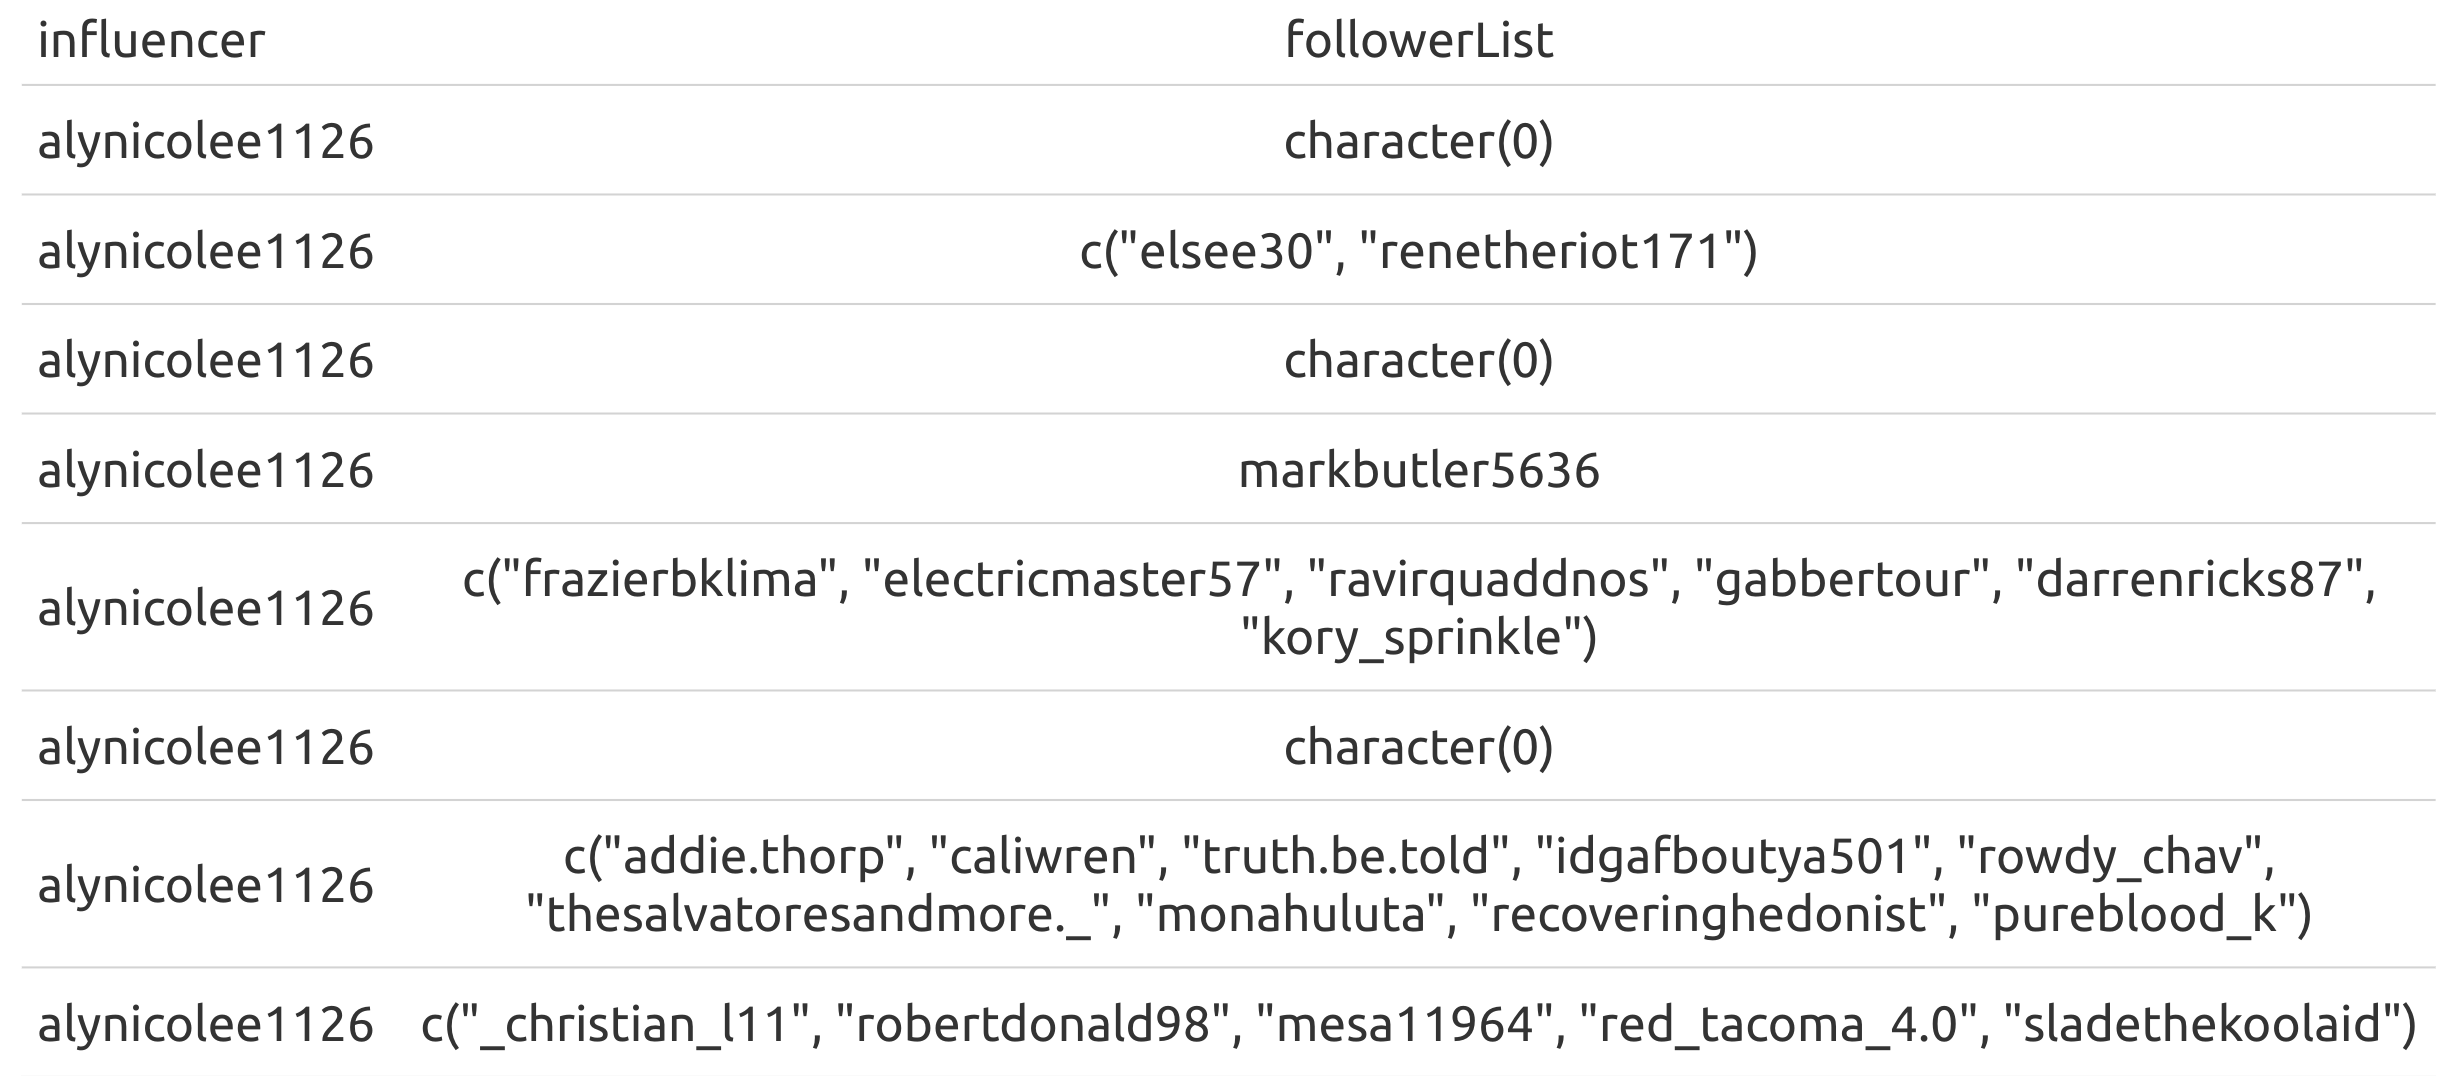
\includegraphics[width = .48\textwidth]{images/total_table_p23.png}

\subsection{Social Graph}
Broadly speaking, a social graph is a graph that represents social relations between entities, were vertices (or nodes) represents users and edges represents relations between such users. It is a model of representation of a social network, and has been referred to as "the global mapping of everybody and how they're related".\\ 
To give a brief example: if Alice and Bob are friends on a social network, in a social graph they would be represented each as a node, and there would be an edge between them.\\
The term was popularized at the Facebook F8 conference on May 24, 2007, when it was used to explain how the newly introduced Facebook Platform would take advantage of the relationships between individuals to offer a richer online experience \cite{wikiSAN}.

\aCapo{}

\includegraphics[width = .5\textwidth]{images/alice_bob_san.png}

Employing a social graph has numerous advantages: it helps visualize all gathered data (all users and their relations), visualize the presence of echo chambers and give insights to analyze the network as a whole. \\
The graph that follows clearly demonstrate that, at least with the gathered data, users do not interact with each other outside their communities, thus forming cliques that can easily be interpreted as echo chambers:
